% Options for packages loaded elsewhere
\PassOptionsToPackage{unicode}{hyperref}
\PassOptionsToPackage{hyphens}{url}
%
\documentclass[
  12pt,
]{article}
\usepackage{amsmath,amssymb}
\usepackage{lmodern}
\usepackage{iftex}
\ifPDFTeX
  \usepackage[T1]{fontenc}
  \usepackage[utf8]{inputenc}
  \usepackage{textcomp} % provide euro and other symbols
\else % if luatex or xetex
  \usepackage{unicode-math}
  \defaultfontfeatures{Scale=MatchLowercase}
  \defaultfontfeatures[\rmfamily]{Ligatures=TeX,Scale=1}
\fi
% Use upquote if available, for straight quotes in verbatim environments
\IfFileExists{upquote.sty}{\usepackage{upquote}}{}
\IfFileExists{microtype.sty}{% use microtype if available
  \usepackage[]{microtype}
  \UseMicrotypeSet[protrusion]{basicmath} % disable protrusion for tt fonts
}{}
\makeatletter
\@ifundefined{KOMAClassName}{% if non-KOMA class
  \IfFileExists{parskip.sty}{%
    \usepackage{parskip}
  }{% else
    \setlength{\parindent}{0pt}
    \setlength{\parskip}{6pt plus 2pt minus 1pt}}
}{% if KOMA class
  \KOMAoptions{parskip=half}}
\makeatother
\usepackage{xcolor}
\IfFileExists{xurl.sty}{\usepackage{xurl}}{} % add URL line breaks if available
\IfFileExists{bookmark.sty}{\usepackage{bookmark}}{\usepackage{hyperref}}
\hypersetup{
  pdftitle={The cbcTools Package: Tools for Designing and Testing Choice-Based Conjoint Surveys in R},
  pdfauthor={John Paul Helveston, Ph.D.},
  hidelinks,
  pdfcreator={LaTeX via pandoc}}
\urlstyle{same} % disable monospaced font for URLs
\usepackage[margin=1in]{geometry}
\usepackage{color}
\usepackage{fancyvrb}
\newcommand{\VerbBar}{|}
\newcommand{\VERB}{\Verb[commandchars=\\\{\}]}
\DefineVerbatimEnvironment{Highlighting}{Verbatim}{commandchars=\\\{\}}
% Add ',fontsize=\small' for more characters per line
\usepackage{framed}
\definecolor{shadecolor}{RGB}{248,248,248}
\newenvironment{Shaded}{\begin{snugshade}}{\end{snugshade}}
\newcommand{\AlertTok}[1]{\textcolor[rgb]{0.94,0.16,0.16}{#1}}
\newcommand{\AnnotationTok}[1]{\textcolor[rgb]{0.56,0.35,0.01}{\textbf{\textit{#1}}}}
\newcommand{\AttributeTok}[1]{\textcolor[rgb]{0.77,0.63,0.00}{#1}}
\newcommand{\BaseNTok}[1]{\textcolor[rgb]{0.00,0.00,0.81}{#1}}
\newcommand{\BuiltInTok}[1]{#1}
\newcommand{\CharTok}[1]{\textcolor[rgb]{0.31,0.60,0.02}{#1}}
\newcommand{\CommentTok}[1]{\textcolor[rgb]{0.56,0.35,0.01}{\textit{#1}}}
\newcommand{\CommentVarTok}[1]{\textcolor[rgb]{0.56,0.35,0.01}{\textbf{\textit{#1}}}}
\newcommand{\ConstantTok}[1]{\textcolor[rgb]{0.00,0.00,0.00}{#1}}
\newcommand{\ControlFlowTok}[1]{\textcolor[rgb]{0.13,0.29,0.53}{\textbf{#1}}}
\newcommand{\DataTypeTok}[1]{\textcolor[rgb]{0.13,0.29,0.53}{#1}}
\newcommand{\DecValTok}[1]{\textcolor[rgb]{0.00,0.00,0.81}{#1}}
\newcommand{\DocumentationTok}[1]{\textcolor[rgb]{0.56,0.35,0.01}{\textbf{\textit{#1}}}}
\newcommand{\ErrorTok}[1]{\textcolor[rgb]{0.64,0.00,0.00}{\textbf{#1}}}
\newcommand{\ExtensionTok}[1]{#1}
\newcommand{\FloatTok}[1]{\textcolor[rgb]{0.00,0.00,0.81}{#1}}
\newcommand{\FunctionTok}[1]{\textcolor[rgb]{0.00,0.00,0.00}{#1}}
\newcommand{\ImportTok}[1]{#1}
\newcommand{\InformationTok}[1]{\textcolor[rgb]{0.56,0.35,0.01}{\textbf{\textit{#1}}}}
\newcommand{\KeywordTok}[1]{\textcolor[rgb]{0.13,0.29,0.53}{\textbf{#1}}}
\newcommand{\NormalTok}[1]{#1}
\newcommand{\OperatorTok}[1]{\textcolor[rgb]{0.81,0.36,0.00}{\textbf{#1}}}
\newcommand{\OtherTok}[1]{\textcolor[rgb]{0.56,0.35,0.01}{#1}}
\newcommand{\PreprocessorTok}[1]{\textcolor[rgb]{0.56,0.35,0.01}{\textit{#1}}}
\newcommand{\RegionMarkerTok}[1]{#1}
\newcommand{\SpecialCharTok}[1]{\textcolor[rgb]{0.00,0.00,0.00}{#1}}
\newcommand{\SpecialStringTok}[1]{\textcolor[rgb]{0.31,0.60,0.02}{#1}}
\newcommand{\StringTok}[1]{\textcolor[rgb]{0.31,0.60,0.02}{#1}}
\newcommand{\VariableTok}[1]{\textcolor[rgb]{0.00,0.00,0.00}{#1}}
\newcommand{\VerbatimStringTok}[1]{\textcolor[rgb]{0.31,0.60,0.02}{#1}}
\newcommand{\WarningTok}[1]{\textcolor[rgb]{0.56,0.35,0.01}{\textbf{\textit{#1}}}}
\usepackage{longtable,booktabs,array}
\usepackage{calc} % for calculating minipage widths
% Correct order of tables after \paragraph or \subparagraph
\usepackage{etoolbox}
\makeatletter
\patchcmd\longtable{\par}{\if@noskipsec\mbox{}\fi\par}{}{}
\makeatother
% Allow footnotes in longtable head/foot
\IfFileExists{footnotehyper.sty}{\usepackage{footnotehyper}}{\usepackage{footnote}}
\makesavenoteenv{longtable}
\usepackage{graphicx}
\makeatletter
\def\maxwidth{\ifdim\Gin@nat@width>\linewidth\linewidth\else\Gin@nat@width\fi}
\def\maxheight{\ifdim\Gin@nat@height>\textheight\textheight\else\Gin@nat@height\fi}
\makeatother
% Scale images if necessary, so that they will not overflow the page
% margins by default, and it is still possible to overwrite the defaults
% using explicit options in \includegraphics[width, height, ...]{}
\setkeys{Gin}{width=\maxwidth,height=\maxheight,keepaspectratio}
% Set default figure placement to htbp
\makeatletter
\def\fps@figure{htbp}
\makeatother
\setlength{\emergencystretch}{3em} % prevent overfull lines
\providecommand{\tightlist}{%
  \setlength{\itemsep}{0pt}\setlength{\parskip}{0pt}}
\setcounter{secnumdepth}{-\maxdimen} % remove section numbering
\usepackage{booktabs}
\usepackage{longtable}
\usepackage{array}
\usepackage{multirow}
\usepackage{wrapfig}
\usepackage{float}
\usepackage{colortbl}
\usepackage{pdflscape}
\usepackage{tabu}
\usepackage{threeparttable}
\usepackage{threeparttablex}
\usepackage[normalem]{ulem}
\usepackage{makecell}
\usepackage{xcolor}
\ifLuaTeX
  \usepackage{selnolig}  % disable illegal ligatures
\fi

\title{The cbcTools Package: Tools for Designing and Testing
Choice-Based Conjoint Surveys in R}
\author{John Paul Helveston, Ph.D.\footnote{Engineering Management and
  Systems Engineering, George Washington University, Washington, D.C.
  USA}}
\date{}

\begin{document}
\maketitle
\begin{abstract}
Traditional tools for designing choice-based conjoint survey experiments
focus on optimizing the design of experiment for statistical power under
ideal conditions. But these tools rarely provide guidance on important
design decisions for less ideal conditions, such as when preference
heterogeneity may be expected in respondent choices or when strong
interactions may be expected between certain attributes. The
\texttt{cbcTools} R package was developed to provide researchers tools
for creating and assessing experiment designs and sample size
requirements under a variety of different conditions prior to fielding
an experiment. The package contains functions for generating experiment
designs and surveys as well as functions for simulating choice data and
conducting power analyses. Since the package data format matches that of
designs exported from Sawtooth Software, it should integrate into the
Sawtooth workflow. Detailed package documentation can be found at
\url{https://jhelvy.github.io/cbcTools/}.
\end{abstract}

Designing a choice-based conjoint survey is almost never a simple,
straightforward process. Designers must consider multiple trade offs
between design parameters (e.g., which attributes and levels to include,
how many choice questions to ask each respondent, and how many
alternatives per choice question) and the design outcomes in terms of
the user experience and the statistical power available for identifying
effects. The process is typically highly iterative.

As a quick example, consider a simple conjoint experiment about cars
with just two attributes (``Price'' and ``Brand'') with the levels in
the table below:

\begin{table}

\caption{\label{tab:unnamed-chunk-1}Example conjoint attributes and levels.}
\centering
\begin{tabular}[t]{ll}
\toprule
Attribute & Levels\\
\midrule
Brand & GM, BMW, Ferrari\\
Price & \$20,000, \$40,000, \$100,000\\
\bottomrule
\end{tabular}
\end{table}

A simple starting point is to generate a design by randomly choosing
combinations of brands and prices from the full set of all possible
profiles. Once created, one of the first things designers examine is the
count of how often each level of each attribute is shown. The table
below shows an example of the counts from a random design with 9 choice
sets of 3 alternatives per question:

\begin{table}

\caption{\label{tab:unnamed-chunk-2}Example conjoint attributes and levels.}
\centering
\begin{tabular}[t]{}
\toprule

\bottomrule
\end{tabular}
\end{table}

\begin{verbatim}
Pairwise attribute counts:

brand & price:

                   Price
                 | 20k 40k 100k
                 |  9   9    9
    Brand        |--------------
    GM        10 |  3   0    7
    BMW       11 |  4   5    2
    Ferrari    6 |  2   4    0
\end{verbatim}

Based on the counts alone, it is clear that this design has several
problems. First, while the price levels are perfectly balanced (each
level is shown 9 times), the brand levels are not -- GW and BMW are
shown 10 and 11 times, respectively, whereas Ferrari is only shown 6
times. But the pairwise counts are particularly troubling. The Ferrari
brand is only shown with a price of \$20,000 and \$40,000 and never at
the \$100,000 level (the most logical level for a Ferrari!). Likewise,
GM brand is shown with a price of \$100,000 in 7 out of 10 times and
never with a price of \$40,000.

This rather poor design is a common outcome when using a randomized
design with a small number of choice sets. Simply increasing the number
of choice sets often results in a much better balance. For example, if
we increase the number from 9 to 90, we obtain the following counts:

\begin{verbatim}
Pairwise attribute counts:

brand & price:

                   Price
                 | 20k 40k 100k
                 |  91  84   95
    Brand        |--------------
    GM        92 |  31  31   30
    BMW       80 |  25  25   30
    Ferrari   98 |  35  28   35
\end{verbatim}

This design has a much better balance across the attribute levels than
the one created from just 9 choice sets. However, it too has issues.
Consider, for example, that about 1/3 of the time the Ferrari brand is
shown it has a price of just \$20,000. This is obviously an unrealistic
profile, and if a user saw such a profile multiple times they may not
take the choice exercise seriously.

One approach to try to correct this outcome is to use a Bayesian
D-efficient design. This approach allows the designer to list a set of
priors on the expected coefficients for each attribute level and then
use an algorithm to select combinations of profiles that maximize the
information available to identify main effects.

\begin{table}

\caption{\label{tab:unnamed-chunk-3}Example conjoint attributes and levels.}
\centering
\begin{tabular}[t]{llr}
\toprule
Attribute & Level & Prior..utility.\\
\midrule
**Price** & \$20,000 & 0\\
 & \$40,000 & -1\\
 & \$100,000 & -4\\
**Brand** & GM & 0\\
 & BMW & 1\\
\addlinespace
 & Ferrari & 2\\
\bottomrule
\end{tabular}
\end{table}

\begin{verbatim}
Attribute counts:

brand:
  GM    BMW   Ferrari 
  93    90     86

price:

  20k  40k 100k 
  97   93   78
\end{verbatim}

\begin{verbatim}
Pairwise attribute counts:

brand & price:
         
          20k 40k 100k
  GM      52  41  0
  BMW     30  30  30
  Ferrari 15  22  49
\end{verbatim}

\hypertarget{centerbayesian-d-efficient-designs}{%
\section{.center{[}Bayesian D-efficient
designs{]}}\label{centerbayesian-d-efficient-designs}}

\hypertarget{centerattempts-to-maximize-information-on-.redmain-effects}{%
\subsubsection{.center{[}Attempts to maximize information on .red{[}Main
Effects{]}{]}}\label{centerattempts-to-maximize-information-on-.redmain-effects}}

``images/design\_compare.png''

\hypertarget{centerbut-.redinteraction-effects-are-confounded-in-d-efficient-designs}{%
\subsubsection{.center{[}\ldots but .red{[}interaction effects{]} are
confounded in D-efficient
designs{]}}\label{centerbut-.redinteraction-effects-are-confounded-in-d-efficient-designs}}

``images/design\_compare\_int.png''

\hypertarget{centerbut-what-about-other-factors}{%
\section{.center{[}But what about other
factors?{]}}\label{centerbut-what-about-other-factors}}

\begin{itemize}
\tightlist
\item
  What if I add one more choice question to each respondent?
\item
  What if I increase the number of alternatives per choice question?
\item
  What if I use a labeled design (aka ``alternative-specific design'')?
\item
  What if there are interaction effects?
\end{itemize}

This paper introduces a package designed for this purpose.

The \texttt{cbcTools} package provides a set of tools for designing
surveys and conducting power analyses for choice-based conjoint survey
experiments in R. The package is designed as a series of functions (each
starting with \texttt{cbc\_}) that are designed to work in sequence
through the

Often times the Traditional tools for designing choice-based conjoint
survey experiments focus on optimizing the design of experiment for
statistical power under ideal conditions. But these tools rarely provide
guidance on important design decisions for less ideal conditions, such
as when preference heterogeneity may be expected in respondent choices
or when strong interactions may be expected between certain attributes.
The \texttt{cbcTools} R package was developed to provide researchers
tools for creating and assessing experiment designs and sample size
requirements under a variety of different conditions prior to fielding
an experiment. The package contains functions for generating experiment
designs and surveys as well as functions for simulating choice data and
conducting power analyses. Since the package data format matches that of
designs exported from Sawtooth Software, it should integrate into the
Sawtooth workflow. Detailed package documentation can be found at
\url{https://jhelvy.github.io/cbcTools/}.

\hypertarget{make-survey-designs}{%
\subsection{Make survey designs}\label{make-survey-designs}}

\hypertarget{generating-profiles}{%
\subsubsection{Generating profiles}\label{generating-profiles}}

The first step in designing an experiment is to define the attributes
and levels for your experiment and then generate all of the
\texttt{profiles} of each possible combination of those attributes and
levels. For example, let's say you're designing a conjoint experiment
about apples and you want to include \texttt{price}, \texttt{type}, and
\texttt{freshness} as attributes. You can obtain all of the possible
profiles for these attributes using the \texttt{cbc\_profiles()}
function:

\begin{Shaded}
\begin{Highlighting}[]
\NormalTok{profiles }\OtherTok{\textless{}{-}} \FunctionTok{cbc\_profiles}\NormalTok{(}
  \AttributeTok{price     =} \FunctionTok{seq}\NormalTok{(}\DecValTok{1}\NormalTok{, }\DecValTok{4}\NormalTok{, }\FloatTok{0.5}\NormalTok{), }\CommentTok{\# $ per pound}
  \AttributeTok{type      =} \FunctionTok{c}\NormalTok{(}\StringTok{\textquotesingle{}Fuji\textquotesingle{}}\NormalTok{, }\StringTok{\textquotesingle{}Gala\textquotesingle{}}\NormalTok{, }\StringTok{\textquotesingle{}Honeycrisp\textquotesingle{}}\NormalTok{),}
  \AttributeTok{freshness =} \FunctionTok{c}\NormalTok{(}\StringTok{\textquotesingle{}Poor\textquotesingle{}}\NormalTok{, }\StringTok{\textquotesingle{}Average\textquotesingle{}}\NormalTok{, }\StringTok{\textquotesingle{}Excellent\textquotesingle{}}\NormalTok{)}
\NormalTok{)}

\FunctionTok{nrow}\NormalTok{(profiles)}
\end{Highlighting}
\end{Shaded}

\begin{verbatim}
#> [1] 63
\end{verbatim}

\begin{Shaded}
\begin{Highlighting}[]
\FunctionTok{head}\NormalTok{(profiles)}
\end{Highlighting}
\end{Shaded}

\begin{verbatim}
#>   profileID price type freshness
#> 1         1   1.0 Fuji      Poor
#> 2         2   1.5 Fuji      Poor
#> 3         3   2.0 Fuji      Poor
#> 4         4   2.5 Fuji      Poor
#> 5         5   3.0 Fuji      Poor
#> 6         6   3.5 Fuji      Poor
\end{verbatim}

\begin{Shaded}
\begin{Highlighting}[]
\FunctionTok{tail}\NormalTok{(profiles)}
\end{Highlighting}
\end{Shaded}

\begin{verbatim}
#>    profileID price       type freshness
#> 58        58   1.5 Honeycrisp Excellent
#> 59        59   2.0 Honeycrisp Excellent
#> 60        60   2.5 Honeycrisp Excellent
#> 61        61   3.0 Honeycrisp Excellent
#> 62        62   3.5 Honeycrisp Excellent
#> 63        63   4.0 Honeycrisp Excellent
\end{verbatim}

Depending on the context of your survey, you may wish to eliminate or
modify some profiles before designing your conjoint survey (e.g., some
profile combinations may be illogical or unrealistic). \textbf{WARNING:
including hard constraints in your designs can substantially reduce the
statistical power of your design, so use them cautiously and avoid them
if possible}.

If you do wish to set some levels conditional on those of other
attributes, you can do so by setting each level of an attribute to a
list that defines these constraints. In the example below, the
\texttt{type} attribute has constraints such that only certain price
levels will be shown for each level. In addition, for the
\texttt{"Honeycrisp"} level, only two of the three \texttt{freshness}
levels are included: \texttt{"Excellent"} and \texttt{"Average"}. Note
that both the other attributes (\texttt{price} and \texttt{freshness})
should contain all of the possible levels. When these constraints you
can see that there are only 30 profiles compared to 63 without
constraints:

\begin{Shaded}
\begin{Highlighting}[]
\NormalTok{profiles }\OtherTok{\textless{}{-}} \FunctionTok{cbc\_profiles}\NormalTok{(}
  \AttributeTok{price =} \FunctionTok{c}\NormalTok{(}\DecValTok{1}\NormalTok{, }\FloatTok{1.5}\NormalTok{, }\DecValTok{2}\NormalTok{, }\FloatTok{2.5}\NormalTok{, }\DecValTok{3}\NormalTok{, }\FloatTok{3.5}\NormalTok{, }\DecValTok{4}\NormalTok{, }\FloatTok{4.5}\NormalTok{, }\DecValTok{5}\NormalTok{),}
  \AttributeTok{freshness =} \FunctionTok{c}\NormalTok{(}\StringTok{\textquotesingle{}Poor\textquotesingle{}}\NormalTok{, }\StringTok{\textquotesingle{}Average\textquotesingle{}}\NormalTok{, }\StringTok{\textquotesingle{}Excellent\textquotesingle{}}\NormalTok{),}
  \AttributeTok{type =} \FunctionTok{list}\NormalTok{(}
    \StringTok{"Fuji"} \OtherTok{=} \FunctionTok{list}\NormalTok{(}
        \AttributeTok{price =} \FunctionTok{c}\NormalTok{(}\DecValTok{2}\NormalTok{, }\FloatTok{2.5}\NormalTok{, }\DecValTok{3}\NormalTok{)}
\NormalTok{    ),}
    \StringTok{"Gala"} \OtherTok{=} \FunctionTok{list}\NormalTok{(}
        \AttributeTok{price =} \FunctionTok{c}\NormalTok{(}\DecValTok{1}\NormalTok{, }\FloatTok{1.5}\NormalTok{, }\DecValTok{2}\NormalTok{)}
\NormalTok{    ),}
    \StringTok{"Honeycrisp"} \OtherTok{=} \FunctionTok{list}\NormalTok{(}
        \AttributeTok{price =} \FunctionTok{c}\NormalTok{(}\FloatTok{2.5}\NormalTok{, }\DecValTok{3}\NormalTok{, }\FloatTok{3.5}\NormalTok{, }\DecValTok{4}\NormalTok{, }\FloatTok{4.5}\NormalTok{, }\DecValTok{5}\NormalTok{),}
        \AttributeTok{freshness =} \FunctionTok{c}\NormalTok{(}\StringTok{"Average"}\NormalTok{, }\StringTok{"Excellent"}\NormalTok{)}
\NormalTok{    )}
\NormalTok{  )}
\NormalTok{)}

\FunctionTok{nrow}\NormalTok{(profiles)}
\end{Highlighting}
\end{Shaded}

\begin{verbatim}
#> [1] 30
\end{verbatim}

\begin{Shaded}
\begin{Highlighting}[]
\FunctionTok{head}\NormalTok{(profiles)}
\end{Highlighting}
\end{Shaded}

\begin{verbatim}
#>   profileID price freshness type
#> 1         1   2.0      Poor Fuji
#> 2         2   2.5      Poor Fuji
#> 3         3   3.0      Poor Fuji
#> 4         4   2.0   Average Fuji
#> 5         5   2.5   Average Fuji
#> 6         6   3.0   Average Fuji
\end{verbatim}

\begin{Shaded}
\begin{Highlighting}[]
\FunctionTok{tail}\NormalTok{(profiles)}
\end{Highlighting}
\end{Shaded}

\begin{verbatim}
#>    profileID price freshness       type
#> 25        25   2.5 Excellent Honeycrisp
#> 26        26   3.0 Excellent Honeycrisp
#> 27        27   3.5 Excellent Honeycrisp
#> 28        28   4.0 Excellent Honeycrisp
#> 29        29   4.5 Excellent Honeycrisp
#> 30        30   5.0 Excellent Honeycrisp
\end{verbatim}

\hypertarget{generating-random-designs}{%
\subsubsection{Generating random
designs}\label{generating-random-designs}}

Once a set of profiles is obtained, a randomized conjoint survey can
then be generated using the \texttt{cbc\_design()} function:

\begin{Shaded}
\begin{Highlighting}[]
\NormalTok{design }\OtherTok{\textless{}{-}} \FunctionTok{cbc\_design}\NormalTok{(}
  \AttributeTok{profiles =}\NormalTok{ profiles,}
  \AttributeTok{n\_resp   =} \DecValTok{900}\NormalTok{, }\CommentTok{\# Number of respondents}
  \AttributeTok{n\_alts   =} \DecValTok{3}\NormalTok{,   }\CommentTok{\# Number of alternatives per question}
  \AttributeTok{n\_q      =} \DecValTok{6}    \CommentTok{\# Number of questions per respondent}
\NormalTok{)}

\FunctionTok{dim}\NormalTok{(design)  }\CommentTok{\# View dimensions}
\end{Highlighting}
\end{Shaded}

\begin{verbatim}
#> [1] 16200     8
\end{verbatim}

\begin{Shaded}
\begin{Highlighting}[]
\FunctionTok{head}\NormalTok{(design) }\CommentTok{\# Preview first 6 rows}
\end{Highlighting}
\end{Shaded}

\begin{verbatim}
#>   respID qID altID obsID profileID price       type freshness
#> 1      1   1     1     1         9   1.5       Gala      Poor
#> 2      1   1     2     1        58   1.5 Honeycrisp Excellent
#> 3      1   1     3     1         3   2.0       Fuji      Poor
#> 4      1   2     1     2        39   2.5 Honeycrisp   Average
#> 5      1   2     2     2        38   2.0 Honeycrisp   Average
#> 6      1   2     3     2        58   1.5 Honeycrisp Excellent
\end{verbatim}

For now, the \texttt{cbc\_design()} function only generates a randomized
design. Other packages, such as the
\href{https://github.com/traets/idefix}{\{idefix\}} package, are able to
generate other types of designs, such as Bayesian D-efficient designs.
The randomized design simply samples from the set of \texttt{profiles}.
It also ensures that no two profiles are the same in any choice
question.

The resulting \texttt{design} data frame includes the following columns:

\begin{itemize}
\tightlist
\item
  \texttt{respID}: Identifies each survey respondent.
\item
  \texttt{qID}: Identifies the choice question answered by the
  respondent.
\item
  \texttt{altID}:Identifies the alternative in any one choice
  observation.
\item
  \texttt{obsID}: Identifies each unique choice observation across all
  respondents.
\item
  \texttt{profileID}: Identifies the profile in \texttt{profiles}.
\end{itemize}

\hypertarget{labeled-designs-a.k.a.-alternative-specific-designs}{%
\subsubsection{Labeled designs (a.k.a. ``alternative-specific''
designs)}\label{labeled-designs-a.k.a.-alternative-specific-designs}}

You can also make a ``labeled'' design (also known as
``alternative-specific'' design) where the levels of one attribute is
used as a label by setting the \texttt{label} argument to that
attribute. This by definition sets the number of alternatives in each
question to the number of levels in the chosen attribute, so the
\texttt{n\_alts} argument is overridden. Here is an example labeled
survey using the \texttt{type} attribute as the label:

\begin{Shaded}
\begin{Highlighting}[]
\NormalTok{design\_labeled }\OtherTok{\textless{}{-}} \FunctionTok{cbc\_design}\NormalTok{(}
  \AttributeTok{profiles  =}\NormalTok{ profiles,}
  \AttributeTok{n\_resp    =} \DecValTok{900}\NormalTok{, }\CommentTok{\# Number of respondents}
  \AttributeTok{n\_alts    =} \DecValTok{3}\NormalTok{,   }\CommentTok{\# Number of alternatives per question}
  \AttributeTok{n\_q       =} \DecValTok{6}\NormalTok{,   }\CommentTok{\# Number of questions per respondent}
  \AttributeTok{label     =} \StringTok{"type"} \CommentTok{\# Set the "type" attribute as the label}
\NormalTok{)}

\FunctionTok{dim}\NormalTok{(design\_labeled)}
\end{Highlighting}
\end{Shaded}

\begin{verbatim}
#> [1] 16200     8
\end{verbatim}

\begin{Shaded}
\begin{Highlighting}[]
\FunctionTok{head}\NormalTok{(design\_labeled)}
\end{Highlighting}
\end{Shaded}

\begin{verbatim}
#>   respID qID altID obsID profileID price       type freshness
#> 1      1   1     1     1         7   4.0       Fuji      Poor
#> 2      1   1     2     1        33   3.0       Gala   Average
#> 3      1   1     3     1        21   4.0 Honeycrisp      Poor
#> 4      1   2     1     2        43   1.0       Fuji Excellent
#> 5      1   2     2     2        52   2.0       Gala Excellent
#> 6      1   2     3     2        16   1.5 Honeycrisp      Poor
\end{verbatim}

In the above example, you can see in the first six rows of the survey
that the \texttt{type} attribute is always fixed to be the same order,
ensuring that each level in the \texttt{type} attribute will always be
shown in each choice question.

\hypertarget{adding-a-no-choice-option-a.k.a.-outside-good}{%
\subsubsection{Adding a ``no choice'' option (a.k.a. ``outside
good'')}\label{adding-a-no-choice-option-a.k.a.-outside-good}}

You can include a ``no choice'' (also known as ``outside good'' option
in your survey by setting \texttt{no\_choice\ =\ TRUE}. If included, all
categorical attributes will be dummy-coded to appropriately dummy-code
the ``no choice'' alternative.

\begin{Shaded}
\begin{Highlighting}[]
\NormalTok{design\_nochoice }\OtherTok{\textless{}{-}} \FunctionTok{cbc\_design}\NormalTok{(}
  \AttributeTok{profiles  =}\NormalTok{ profiles,}
  \AttributeTok{n\_resp    =} \DecValTok{900}\NormalTok{, }\CommentTok{\# Number of respondents}
  \AttributeTok{n\_alts    =} \DecValTok{3}\NormalTok{, }\CommentTok{\# Number of alternatives per question}
  \AttributeTok{n\_q       =} \DecValTok{6}\NormalTok{, }\CommentTok{\# Number of questions per respondent}
  \AttributeTok{no\_choice =} \ConstantTok{TRUE}
\NormalTok{)}

\FunctionTok{dim}\NormalTok{(design\_nochoice)}
\end{Highlighting}
\end{Shaded}

\begin{verbatim}
#> [1] 21600    13
\end{verbatim}

\begin{Shaded}
\begin{Highlighting}[]
\FunctionTok{head}\NormalTok{(design\_nochoice)}
\end{Highlighting}
\end{Shaded}

\begin{verbatim}
#>   respID qID altID obsID profileID price type_Fuji type_Gala type_Honeycrisp
#> 1      1   1     1     1        41   3.5         0         0               1
#> 2      1   1     2     1        44   1.5         1         0               0
#> 3      1   1     3     1        19   3.0         0         0               1
#> 4      1   1     4     1         0   0.0         0         0               0
#> 5      1   2     1     2        17   2.0         0         0               1
#> 6      1   2     2     2        26   3.0         1         0               0
#>   freshness_Poor freshness_Average freshness_Excellent no_choice
#> 1              0                 1                   0         0
#> 2              0                 0                   1         0
#> 3              1                 0                   0         0
#> 4              0                 0                   0         1
#> 5              1                 0                   0         0
#> 6              0                 1                   0         0
\end{verbatim}

\hypertarget{inspecting-survey-designs}{%
\subsection{Inspecting survey designs}\label{inspecting-survey-designs}}

The package includes some functions to quickly inspect some basic
metrics of a design.

The \texttt{cbc\_balance()} function prints out a summary of the counts
of each level for each attribute across all choice questions as well as
the two-way counts across all pairs of attributes for a given design:

\begin{Shaded}
\begin{Highlighting}[]
\FunctionTok{cbc\_balance}\NormalTok{(design)}
\end{Highlighting}
\end{Shaded}

\begin{verbatim}
#> ==============================
#> price x type 
#> 
#>          Fuji Gala Honeycrisp
#>       NA 5382 5518       5300
#> 1   2322  804  764        754
#> 1.5 2286  745  816        725
#> 2   2275  731  798        746
#> 2.5 2385  771  803        811
#> 3   2290  753  782        755
#> 3.5 2308  787  767        754
#> 4   2334  791  788        755
#> 
#> price x freshness 
#> 
#>          Poor Average Excellent
#>       NA 5378    5398      5424
#> 1   2322  807     775       740
#> 1.5 2286  774     723       789
#> 2   2275  759     767       749
#> 2.5 2385  755     809       821
#> 3   2290  775     730       785
#> 3.5 2308  754     783       771
#> 4   2334  754     811       769
#> 
#> type x freshness 
#> 
#>                 Poor Average Excellent
#>              NA 5378    5398      5424
#> Fuji       5382 1780    1788      1814
#> Gala       5518 1798    1885      1835
#> Honeycrisp 5300 1800    1725      1775
\end{verbatim}

The \texttt{cbc\_overlap()} function prints out a summary of the amount
of ``overlap'' across attributes within the choice questions. For
example, for each attribute, the count under \texttt{"1"} is the number
of choice questions in which the same level was shown across all
alternatives for that attribute (because there was only one level
shown). Likewise, the count under \texttt{"2"} is the number of choice
questions in which only two unique levels of that attribute were shown,
and so on:

\begin{Shaded}
\begin{Highlighting}[]
\FunctionTok{cbc\_overlap}\NormalTok{(design)}
\end{Highlighting}
\end{Shaded}

\begin{verbatim}
#> ==============================
#> Counts of attribute overlap:
#> (# of questions with N unique levels)
#> 
#> price:
#> 
#>    1    2    3 
#>   84 1907 3409 
#> 
#> type:
#> 
#>    1    2    3 
#>  514 3589 1297 
#> 
#> freshness:
#> 
#>    1    2    3 
#>  537 3591 1272
\end{verbatim}

\hypertarget{simulating-choices}{%
\subsection{Simulating choices}\label{simulating-choices}}

You can simulate choices for a given \texttt{design} using the
\texttt{cbc\_choices()} function. By default, random choices are
simulated:

\begin{Shaded}
\begin{Highlighting}[]
\NormalTok{data }\OtherTok{\textless{}{-}} \FunctionTok{cbc\_choices}\NormalTok{(}
  \AttributeTok{design =}\NormalTok{ design,}
  \AttributeTok{obsID  =} \StringTok{"obsID"}
\NormalTok{)}

\FunctionTok{head}\NormalTok{(data)}
\end{Highlighting}
\end{Shaded}

\begin{verbatim}
#>   respID qID altID obsID profileID price       type freshness choice
#> 1      1   1     1     1         9   1.5       Gala      Poor      0
#> 2      1   1     2     1        58   1.5 Honeycrisp Excellent      0
#> 3      1   1     3     1         3   2.0       Fuji      Poor      1
#> 4      1   2     1     2        39   2.5 Honeycrisp   Average      1
#> 5      1   2     2     2        38   2.0 Honeycrisp   Average      0
#> 6      1   2     3     2        58   1.5 Honeycrisp Excellent      0
\end{verbatim}

You can also pass a list of prior parameters to define a utility model
that will be used to simulate choices. In the example below, the choices
are simulated using a utility model with the following parameters:

\begin{itemize}
\tightlist
\item
  1 continuous parameter for \texttt{price}
\item
  2 categorical parameters for \texttt{type}
  (\texttt{\textquotesingle{}Gala\textquotesingle{}} and
  \texttt{\textquotesingle{}Honeycrisp\textquotesingle{}})
\item
  2 categorical parameters for \texttt{freshness} (\texttt{"Average"}
  and \texttt{"Excellent"})
\end{itemize}

Note that for categorical variables (\texttt{type} and
\texttt{freshness} in this example), the first level defined when using
\texttt{cbc\_profiles()} is set as the reference level. The example
below defines the following utility model for simulating choices for
each alternative \emph{j}:

\[
u_j = 0.1price_j + 0.1typeGala_j + 0.2typeHoneycrisp_j + 0.1freshnessAverage_j + 0.2freshnessExcellent_j + \varepsilon_j
\]

\begin{Shaded}
\begin{Highlighting}[]
\NormalTok{data }\OtherTok{\textless{}{-}} \FunctionTok{cbc\_choices}\NormalTok{(}
  \AttributeTok{design =}\NormalTok{ design,}
  \AttributeTok{obsID =} \StringTok{"obsID"}\NormalTok{,}
  \AttributeTok{priors =} \FunctionTok{list}\NormalTok{(}
    \AttributeTok{price     =} \FloatTok{0.1}\NormalTok{,}
    \AttributeTok{type      =} \FunctionTok{c}\NormalTok{(}\FloatTok{0.1}\NormalTok{, }\FloatTok{0.2}\NormalTok{),}
    \AttributeTok{freshness =} \FunctionTok{c}\NormalTok{(}\FloatTok{0.1}\NormalTok{, }\FloatTok{0.2}\NormalTok{)}
\NormalTok{  )}
\NormalTok{)}
\end{Highlighting}
\end{Shaded}

\begin{longtable}[]{@{}ll@{}}
\toprule
Attribute & Level \\
\midrule
\endhead
\textbf{Price} & Continuous \\
\textbf{Type} & Fuji \\
Gala & 0.1 \\
Honeycrisp & 0.2 \\
\textbf{Freshness} & Average \\
Excellent & 0.1 \\
Poor & -0.2 \\
\bottomrule
\end{longtable}

If you wish to include a prior model with an interaction, you can do so
inside the \texttt{priors} list. For example, here is the same example
as above but with an interaction between \texttt{price} and
\texttt{type} added:

\begin{longtable}[]{@{}ll@{}}
\toprule
Attribute & Level \\
\midrule
\endhead
\textbf{Price} & Continuous \\
\textbf{Type} & Fuji \\
Gala & 0.1 \\
Honeycrisp & 0.2 \\
\textbf{Freshness} & Average \\
Excellent & 0.1 \\
Poor & -0.2 \\
\textbf{Price x Type} & Fuji \\
Gala & 0.1 \\
Honeycrisp & 0.5 \\
\bottomrule
\end{longtable}

\begin{Shaded}
\begin{Highlighting}[]
\NormalTok{data }\OtherTok{\textless{}{-}} \FunctionTok{cbc\_choices}\NormalTok{(}
  \AttributeTok{design =}\NormalTok{ design,}
  \AttributeTok{obsID =} \StringTok{"obsID"}\NormalTok{,}
  \AttributeTok{priors =} \FunctionTok{list}\NormalTok{(}
    \AttributeTok{price =} \FloatTok{0.1}\NormalTok{,}
    \AttributeTok{type =} \FunctionTok{c}\NormalTok{(}\FloatTok{0.1}\NormalTok{, }\FloatTok{0.2}\NormalTok{),}
    \AttributeTok{freshness =} \FunctionTok{c}\NormalTok{(}\FloatTok{0.1}\NormalTok{, }\FloatTok{0.2}\NormalTok{),}
    \StringTok{\textasciigrave{}}\AttributeTok{price*type}\StringTok{\textasciigrave{}} \OtherTok{=} \FunctionTok{c}\NormalTok{(}\FloatTok{0.1}\NormalTok{, }\FloatTok{0.5}\NormalTok{)}
\NormalTok{  )}
\NormalTok{)}
\end{Highlighting}
\end{Shaded}

Finally, you can also simulate data for a mixed logit model where
parameters follow a normal or log-normal distribution across the
population. In the example below, the \texttt{randN()} function is used
to specify the \texttt{type} attribute with 2 random normal parameters
with a specified vector of means (\texttt{mean}) and standard deviations
(\texttt{sd}) for each level of \texttt{type}. Log-normal parameters are
specified using \texttt{randLN()}.

\begin{longtable}[]{@{}ll@{}}
\toprule
Attribute & Level \\
\midrule
\endhead
\textbf{Price} & Continuous \\
\textbf{Type} & Fuji \\
Gala & N(0.1, 0.5) \\
Honeycrisp & N(0.2, 1) \\
\textbf{Freshness} & Average \\
Excellent & 0.1 \\
Poor & -0.2 \\
\bottomrule
\end{longtable}

\begin{Shaded}
\begin{Highlighting}[]
\NormalTok{data }\OtherTok{\textless{}{-}} \FunctionTok{cbc\_choices}\NormalTok{(}
  \AttributeTok{design =}\NormalTok{ design,}
  \AttributeTok{obsID =} \StringTok{"obsID"}\NormalTok{,}
  \AttributeTok{priors =} \FunctionTok{list}\NormalTok{(}
    \AttributeTok{price =} \FloatTok{0.1}\NormalTok{,}
    \AttributeTok{type =} \FunctionTok{randN}\NormalTok{(}\AttributeTok{mean =} \FunctionTok{c}\NormalTok{(}\FloatTok{0.1}\NormalTok{, }\FloatTok{0.2}\NormalTok{), }\AttributeTok{sd =} \FunctionTok{c}\NormalTok{(}\DecValTok{1}\NormalTok{, }\DecValTok{2}\NormalTok{)),}
    \AttributeTok{freshness =} \FunctionTok{c}\NormalTok{(}\FloatTok{0.1}\NormalTok{, }\FloatTok{0.2}\NormalTok{)}
\NormalTok{  )}
\NormalTok{)}
\end{Highlighting}
\end{Shaded}

\hypertarget{conducting-a-power-analysis}{%
\subsection{Conducting a power
analysis}\label{conducting-a-power-analysis}}

The simulated choice data can be used to conduct a power analysis by
estimating the same model multiple times with incrementally increasing
sample sizes. As the sample size increases, the estimated coefficient
standard errors will decrease (i.e.~coefficient estimates become more
precise). The \texttt{cbc\_power()} function achieves this by
partitioning the choice data into multiple sizes (defined by the
\texttt{nbreaks} argument) and then estimating a user-defined choice
model on each data subset. In the example below, 10 different sample
sizes are used. All models are estimated using the
\href{https://jhelvy.github.io/logitr}{\{logitr\}} package:

\begin{Shaded}
\begin{Highlighting}[]
\NormalTok{power }\OtherTok{\textless{}{-}} \FunctionTok{cbc\_power}\NormalTok{(}
  \AttributeTok{data    =}\NormalTok{ data,}
  \AttributeTok{pars    =} \FunctionTok{c}\NormalTok{(}\StringTok{"price"}\NormalTok{, }\StringTok{"type"}\NormalTok{, }\StringTok{"freshness"}\NormalTok{),}
  \AttributeTok{outcome =} \StringTok{"choice"}\NormalTok{,}
  \AttributeTok{obsID   =} \StringTok{"obsID"}\NormalTok{,}
  \AttributeTok{nbreaks =} \DecValTok{10}\NormalTok{,}
  \AttributeTok{n\_q     =} \DecValTok{6}
\NormalTok{)}

\FunctionTok{head}\NormalTok{(power)}
\end{Highlighting}
\end{Shaded}

\begin{verbatim}
#>   sampleSize               coef         est         se
#> 1         90              price  0.05889788 0.05180620
#> 2         90           typeGala -0.15581876 0.12818593
#> 3         90     typeHoneycrisp -0.06196309 0.12531121
#> 4         90   freshnessAverage -0.09844676 0.13250000
#> 5         90 freshnessExcellent  0.05163359 0.12719533
#> 6        180              price  0.04710326 0.03711161
\end{verbatim}

\begin{Shaded}
\begin{Highlighting}[]
\FunctionTok{tail}\NormalTok{(power)}
\end{Highlighting}
\end{Shaded}

\begin{verbatim}
#>    sampleSize               coef          est         se
#> 45        810 freshnessExcellent  0.027453970 0.04272986
#> 46        900              price  0.008202336 0.01660304
#> 47        900           typeGala  0.046155661 0.04017443
#> 48        900     typeHoneycrisp -0.002888875 0.04058084
#> 49        900   freshnessAverage  0.044177212 0.04045309
#> 50        900 freshnessExcellent  0.029655335 0.04054307
\end{verbatim}

The \texttt{power} data frame contains the coefficient estimates and
standard errors for each sample size. You can quickly visualize the
outcome to identify a required sample size for a desired level of
parameter precision by using the \texttt{plot()} method:

\begin{Shaded}
\begin{Highlighting}[]
\FunctionTok{plot}\NormalTok{(power)}
\end{Highlighting}
\end{Shaded}

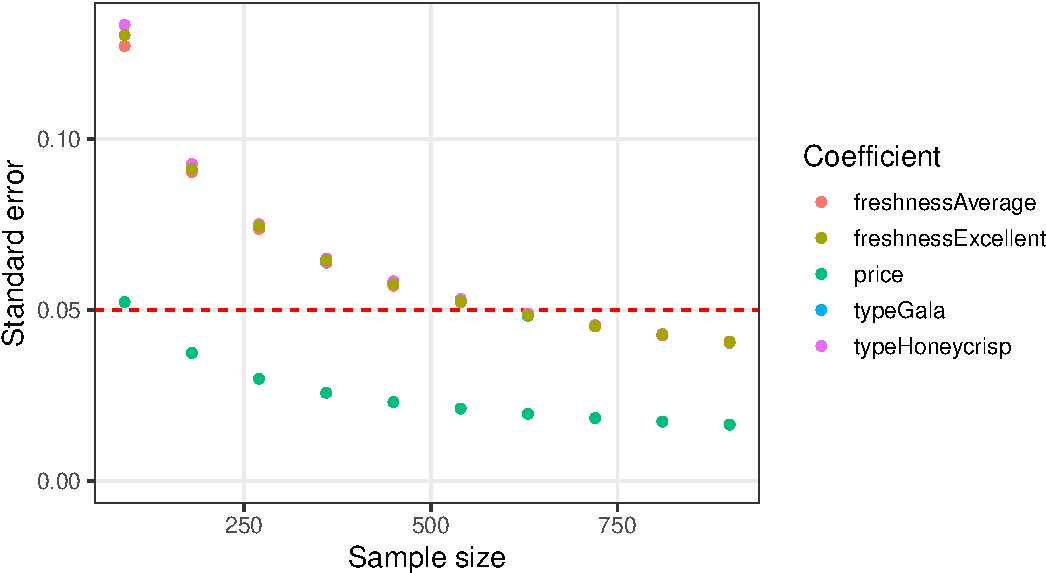
\includegraphics[width=522.144px]{figs/power-1}

If you want to examine any other aspects of the models other than the
standard errors, you can set \texttt{return\_models\ =\ TRUE} and
\texttt{cbc\_power()} will return a list of estimated models. The
example below prints a summary of the last model in the list of models:

\begin{Shaded}
\begin{Highlighting}[]
\FunctionTok{library}\NormalTok{(logitr)}

\NormalTok{models }\OtherTok{\textless{}{-}} \FunctionTok{cbc\_power}\NormalTok{(}
  \AttributeTok{data    =}\NormalTok{ data,}
  \AttributeTok{pars    =} \FunctionTok{c}\NormalTok{(}\StringTok{"price"}\NormalTok{, }\StringTok{"type"}\NormalTok{, }\StringTok{"freshness"}\NormalTok{),}
  \AttributeTok{outcome =} \StringTok{"choice"}\NormalTok{,}
  \AttributeTok{obsID   =} \StringTok{"obsID"}\NormalTok{,}
  \AttributeTok{nbreaks =} \DecValTok{10}\NormalTok{,}
  \AttributeTok{n\_q     =} \DecValTok{6}\NormalTok{,}
  \AttributeTok{return\_models =} \ConstantTok{TRUE}
\NormalTok{)}

\FunctionTok{summary}\NormalTok{(models[[}\DecValTok{10}\NormalTok{]])}
\end{Highlighting}
\end{Shaded}

\begin{verbatim}
#> =================================================
#> Call:
#> FUN(data = X[[i]], outcome = ..1, obsID = ..2, pars = ..3, randPars = ..4, 
#>     panelID = ..5, clusterID = ..6, robust = ..7, predict = ..8)
#> 
#> Frequencies of alternatives:
#>       1       2       3 
#> 0.32389 0.33407 0.34204 
#> 
#> Exit Status: 3, Optimization stopped because ftol_rel or ftol_abs was reached.
#>                                 
#> Model Type:    Multinomial Logit
#> Model Space:          Preference
#> Model Run:                1 of 1
#> Iterations:                    9
#> Elapsed Time:        0h:0m:0.05s
#> Algorithm:        NLOPT_LD_LBFGS
#> Weights Used?:             FALSE
#> Robust?                    FALSE
#> 
#> Model Coefficients: 
#>                      Estimate Std. Error z-value Pr(>|z|)
#> price               0.0082023  0.0166030  0.4940   0.6213
#> typeGala            0.0461557  0.0401744  1.1489   0.2506
#> typeHoneycrisp     -0.0028889  0.0405808 -0.0712   0.9432
#> freshnessAverage    0.0441772  0.0404531  1.0921   0.2748
#> freshnessExcellent  0.0296553  0.0405431  0.7315   0.4645
#>                                      
#> Log-Likelihood:         -5.930800e+03
#> Null Log-Likelihood:    -5.932506e+03
#> AIC:                     1.187160e+04
#> BIC:                     1.190457e+04
#> McFadden R2:             2.876806e-04
#> Adj McFadden R2:        -5.551335e-04
#> Number of Observations:  5.400000e+03
\end{verbatim}

\hypertarget{piping-it-all-together}{%
\subsection{Piping it all together!}\label{piping-it-all-together}}

One of the convenient features of how the package is written is that the
object generated in each step is used as the first argument to the
function for the next step. Thus, just like in the overall program
diagram, the functions can be piped together:

\begin{Shaded}
\begin{Highlighting}[]
\FunctionTok{cbc\_profiles}\NormalTok{(}
  \AttributeTok{price     =} \FunctionTok{seq}\NormalTok{(}\DecValTok{1}\NormalTok{, }\DecValTok{4}\NormalTok{, }\FloatTok{0.5}\NormalTok{), }\CommentTok{\# $ per pound}
  \AttributeTok{type      =} \FunctionTok{c}\NormalTok{(}\StringTok{\textquotesingle{}Fuji\textquotesingle{}}\NormalTok{, }\StringTok{\textquotesingle{}Gala\textquotesingle{}}\NormalTok{, }\StringTok{\textquotesingle{}Honeycrisp\textquotesingle{}}\NormalTok{),}
  \AttributeTok{freshness =} \FunctionTok{c}\NormalTok{(}\StringTok{\textquotesingle{}Poor\textquotesingle{}}\NormalTok{, }\StringTok{\textquotesingle{}Average\textquotesingle{}}\NormalTok{, }\StringTok{\textquotesingle{}Excellent\textquotesingle{}}\NormalTok{)}
\NormalTok{) }\SpecialCharTok{|}\ErrorTok{\textgreater{}}
\FunctionTok{cbc\_design}\NormalTok{(}
  \AttributeTok{n\_resp   =} \DecValTok{900}\NormalTok{, }\CommentTok{\# Number of respondents}
  \AttributeTok{n\_alts   =} \DecValTok{3}\NormalTok{,   }\CommentTok{\# Number of alternatives per question}
  \AttributeTok{n\_q      =} \DecValTok{6}    \CommentTok{\# Number of questions per respondent}
\NormalTok{) }\SpecialCharTok{|}\ErrorTok{\textgreater{}}
\FunctionTok{cbc\_choices}\NormalTok{(}
  \AttributeTok{obsID =} \StringTok{"obsID"}\NormalTok{,}
  \AttributeTok{priors =} \FunctionTok{list}\NormalTok{(}
    \AttributeTok{price     =} \FloatTok{0.1}\NormalTok{,}
    \AttributeTok{type      =} \FunctionTok{c}\NormalTok{(}\FloatTok{0.1}\NormalTok{, }\FloatTok{0.2}\NormalTok{),}
    \AttributeTok{freshness =} \FunctionTok{c}\NormalTok{(}\FloatTok{0.1}\NormalTok{, }\FloatTok{0.2}\NormalTok{)}
\NormalTok{  )}
\NormalTok{) }\SpecialCharTok{|}\ErrorTok{\textgreater{}}
\FunctionTok{cbc\_power}\NormalTok{(}
    \AttributeTok{pars    =} \FunctionTok{c}\NormalTok{(}\StringTok{"price"}\NormalTok{, }\StringTok{"type"}\NormalTok{, }\StringTok{"freshness"}\NormalTok{),}
    \AttributeTok{outcome =} \StringTok{"choice"}\NormalTok{,}
    \AttributeTok{obsID   =} \StringTok{"obsID"}\NormalTok{,}
    \AttributeTok{nbreaks =} \DecValTok{10}\NormalTok{,}
    \AttributeTok{n\_q     =} \DecValTok{6}
\NormalTok{) }\SpecialCharTok{|}\ErrorTok{\textgreater{}}
\FunctionTok{plot}\NormalTok{()}
\end{Highlighting}
\end{Shaded}

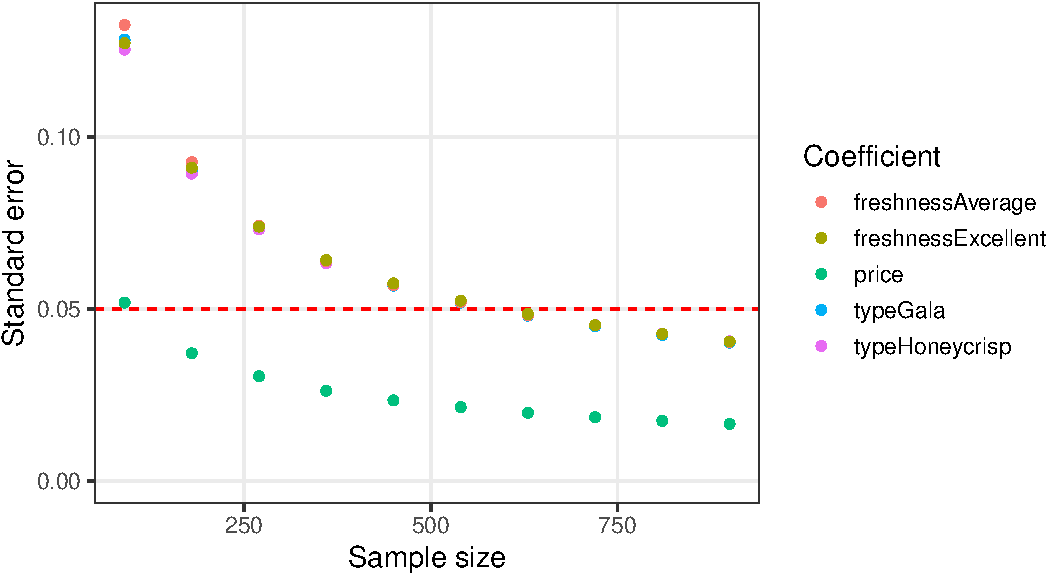
\includegraphics[width=522.144px]{figs/unnamed-chunk-19-1}

\hypertarget{author-version-and-license-information}{%
\subsection{Author, Version, and License
Information}\label{author-version-and-license-information}}

\begin{itemize}
\tightlist
\item
  Author: \emph{John Paul Helveston} \url{https://www.jhelvy.com/}
\item
  Date First Written: \emph{October 23, 2020}
\item
  License:
  \href{https://github.com/jhelvy/cbcTools/blob/master/LICENSE.md}{MIT}
\end{itemize}

\hypertarget{citation-information}{%
\subsection{Citation Information}\label{citation-information}}

If you use this package for in a publication, I would greatly appreciate
it if you cited it - you can get the citation by typing
\texttt{citation("cbcTools")} into R:

\begin{Shaded}
\begin{Highlighting}[]
\FunctionTok{citation}\NormalTok{(}\StringTok{"cbcTools"}\NormalTok{)}
\end{Highlighting}
\end{Shaded}

\begin{verbatim}
#> 
#> To cite cbcTools in publications use:
#> 
#>   John Paul Helveston (2022). cbcTools: Tools For Designing Conjoint
#>   Survey Experiments.
#> 
#> A BibTeX entry for LaTeX users is
#> 
#>   @Manual{,
#>     title = {cbcTools: Tools For Designing Choice-Based Conjoint Survey Experiments},
#>     author = {John Paul Helveston},
#>     year = {2022},
#>     note = {R package version 0.0.3},
#>     url = {https://jhelvy.github.io/cbcTools/},
#>   }
\end{verbatim}

\hypertarget{references}{%
\section*{References}\label{references}}
\addcontentsline{toc}{section}{References}

\end{document}
